
\chapter{Design and Implementation}
\label{ch:impl}
In this chapter, We will dive deeper and learn how the HoneyBadgerBFT works. To have an overview of the protocol, please refer to chapter \ref{ch:hbbft}.
The protocol has four modules, and we will see how each one of them works.

 \begin{table}[!h]
 \centering
\begin{tabular}{ |r|  l| }
\hline
 \textbf{Symbol}& \textbf{Description}  \\
 \hline
HB & HoneyBadger instance\\
RB & Reliable Broadcast instance\\
BA & Binary Agreement instance\\
$N$ & Total number of nodes in the network\\
$f$ & Total number of faulty nodes in the network\\
  \hline
\end{tabular}


  \caption{Notations}
  \end{table}
% \end{center}
\section{Reliable Broadcast}
The purpose of Reliable Broadcast is to broadcast a single node’s contribution to all the nodes in the network.

\begin{figure}[!h]
    \centering
    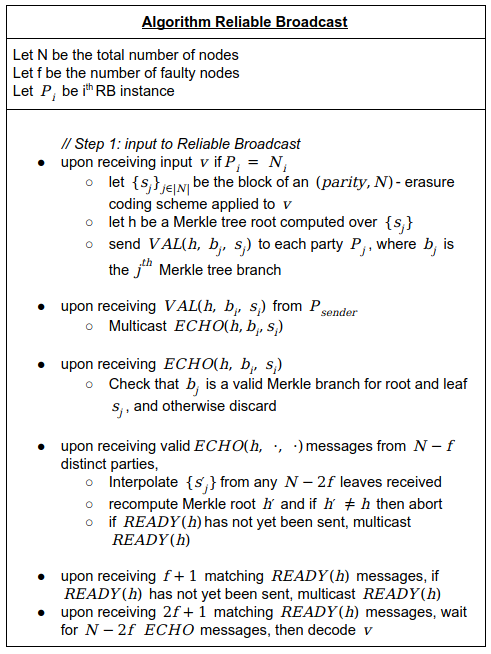
\includegraphics[scale=0.7]{images/rb_algo.png}
    \caption{Reliable broadcast algorithm\cite{miller2016honey}}
    \label{fig:rb_algo}
\end{figure}
\begin{itemize}
    \item Upon receiving a \textit{contribution} from \textit{Subset}, it runs erasure coding scheme to the \textit{contribution} which will return N number of shares.
    \item On these shares, we create a merkle tree with root \textit{h} and send \textit{VAL} message with merkle tree root, merkle tree branch, and share of the \textit{contribution},
   to all the nodes e.g. $i^{th}$ share to $i^{th}$ node.
    \item for \textit{VAL} message,
    \begin{itemize}
        \item Upon receiving \textit{VAL} message, all nodes multi-cast \textit{ECHO} message with same parameters as they received via \textit{VAL} message.
    \end{itemize}
    \item for \textit{ECHO} message,
    \begin{itemize}
        \item upon receiving \textit{ECHO} message, check via merkle tree proof whether this message belongs to the same tree, if not discard the message
        \item Upon receiving $N-f$ distinct valid \textit{ECHO} messages, we try and reconstruct the original contribution, and use merkle tree to verify if the reconstructed message is valid, if not then abort the process.
        \item If \textit{READY(h)} message is not already sent, multi-cast \textit{READY(h)}.
    \end{itemize}
    \item for \textit{READY} message,
    \begin{itemize}
        \item upon receiving at least $f+1$ matching \textit{READY} message, if \textit{READY} is not already sent, then multi-cast \textit{READY(h)}.
        \item upon receiving $2f+1$ matching \textit{READY} messages, wait for $N-2f$ \textit{ECHO} messages, then decode \textit{contribution}. 
    \end{itemize}
\end{itemize}
\section{Binary Agreement}
The purpose of \textit{Binary Agreement} protocol is to determine whether a contribution is to be included in the subset or not, based on the votes from all the nodes.

\begin{figure}[!h]
    \centering
    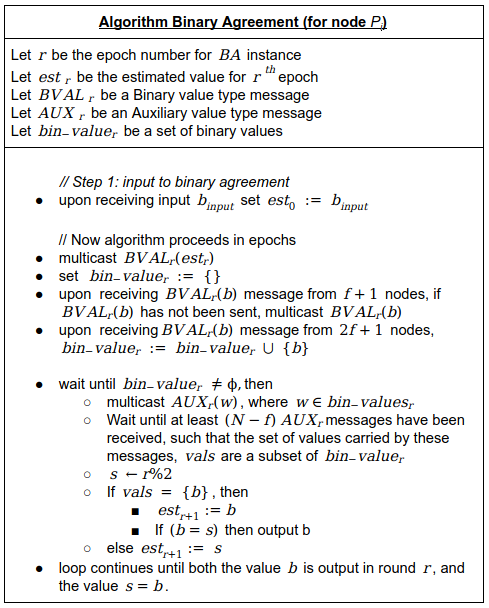
\includegraphics[scale=0.7]{images/ba_algo.png}
    \caption{Binary Agreement algorithm\cite{miller2016honey}}
    \label{fig:ba_algo}
\end{figure}
\begin{itemize}
    \item Binary agreement instance upon getting input sets the estimated value := input value, and starts the first epoch.
    \item In every epoch below given steps are repeated until the binary agreement instance produces an output. $r$ represents the current epoch number.
    \begin{itemize}
        \item we send the $BVAL_{r}(est_{r})$ to all the other nodes.
        \item After receiving $BVAL_{r}(b)$ message from at least $f+1$ nodes, if we have not multi-casted the $BVAL_{r}(b)$ already, we multi-cast it. $f+1$ messages ensures that at least one honest node is vouching for this value.
        \item  After receiving $BVAL_{r}(b)$ message from at least $2f+1$ nodes,
        we add the binary value $b$ to the $bin\_values_r$ set.
        \item Once we have value in the $bin\_values_r$ set, we multi-cast $AUX_{r}(w)$, where $w \in bin\_values_{r}$.
        \item Then we wait to collect at least $(N-f)$ $AUX_{r}$ messages with the value, that is present in the $bin\_values_{r}$ set. Upon receiving sufficient $AUX_{r}$ value we try to produce output for this epoch, before that we set $vals = bin\_values_{r}$ because $bin\_values_{r}$ set can change. 
        \item If we have single value ($b$) in the $vals$ set then the next $est_{r+1} := b$ and if the $b$ equals to the $s$ that is the $r^{th}$ value on common coin then the output of \textit{BA} is $b$, if not we proceed to next epoch.
        \item If we have multiple value in $vals$ then $est_{r+1} := s$ and we proceed to next epoch. 
        \end{itemize}
\end{itemize}
\section{Subset}
This is the main functional unit of the Protocol. Subset receives a contribution from each orderer node and returns subset of contribution agreed by all orderers. 

\begin{figure}[!h]
    \centering
    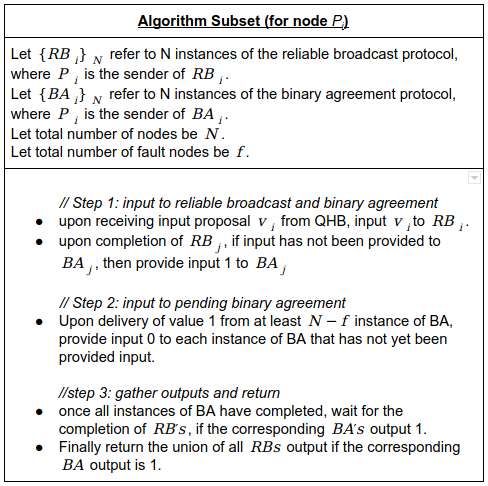
\includegraphics[scale=0.7]{images/subset_algo.png}
    \caption{Subset Algorithm\cite{miller2016honey}}
    \label{fig:subset_algo}
\end{figure}
\begin{figure}[!h]
    \centering
    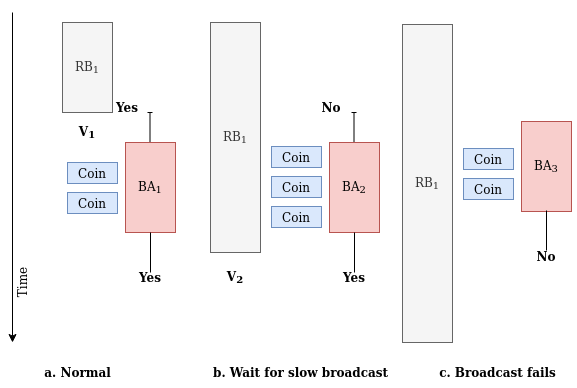
\includegraphics[scale=0.7]{images/subset_illust.png}
    \caption{Illustration of Subset Algorithm}
    \label{fig:subset_illust}
\end{figure}
\begin{itemize}
    \item Each Subset instance have N number of \textit{Reliable Broadcast} instances and N number of \textit{Binary Agreement} instances running under it, representing each node.
    \item Upon receiving input proposal from \textit{HB} it passes the proposal to the \textit{RB} instance corresponding to itself. \textit{RB} instance broadcast the proposal to all the nodes in network. All the other nodes \textit{Subset} instance do the same with their \textit{contribution}.
    \item Upon completion of \textit{RB} protocol, if we have not already provided input to corresponding \textit{BA} instance we provide 1 as input.
    \item Upon completion of $ (N-f) $ \textit{BA} with output as 1, we provide input to all the pending \textit{BA} instances as 0 that has not yet been provided input.
    \item We wait for the \textit{RB} instances to complete, if the corresponding \textit{BA} instance output is 1, refer to figure \ref{fig:subset_illust}.
    \item once all \textit{BA} instances have completed and all \textit{RB} instances either completed or aborted. The results of \textit{RB} instances are combined and returned to \textit{HB}.
\end{itemize}
\section{Honey Badger}
%%TODO HB INTRO
Honey Badger is outer most layer of protocol. It gets tranasction as input from client and return block of ordered transactions.
\begin{figure}[!h]
    \centering
    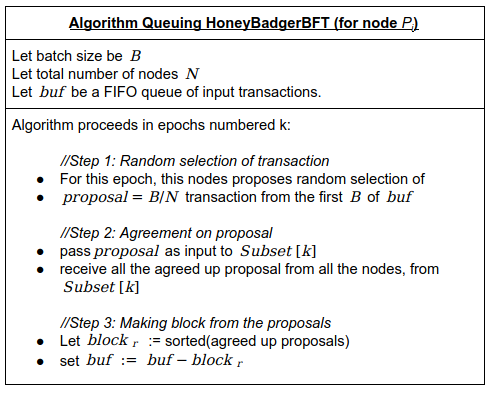
\includegraphics[scale=0.7]{images/qhb_algo.png}
    \caption{Honey Badger Algorithm\cite{miller2016honey}}
    \label{fig:qhb_algo}
\end{figure}
\begin{itemize}
    \item We get transitions as input which are stored in FIFO buffer.
    \item When an \textit{epoch} starts \textit{HB} proposes at most B/N transaction to the \textit{Subset} instance for that epoch. Then it waits  \textit{Subset} for the current \textit{epoch} to complete.
    \item On completion, \textit{Subset} return the proposal for all the nodes that \textit{Subset} has agreed upon.
    \item We sort the proposal e.g. lexicographical order, remove the duplicates, and from a block.
    \item We remove the transaction that are included in the block from the buffer.
    \item Then we return the block and increment the epoch.
\end{itemize}
We have looked at how each module and overall protocol works; in the next section, we will explain implementation details.
\section{Implementation of HoneyBadgerBFT}
We have implemented a stand-alone version of HoneyBadger. We started by understanding, implementing, and testing each module separately and then integrated them, we used Golang for implementation as Hyperladger source code is also in Golang. Our source code for HoneyBadgerBFT is around 2900 LoC.
% with understanding the working of the HoneyBadgerBFT protocol and then implemented it in Golang(around 2900 LoC).

We used following libraries and modules for implementing the protocol:
\begin{itemize}
    \item \href{https://golang.org}{go1.14.2} version of Golang.
    \item \href{https://github.com/klauspost/reedsolomon}{Reed-Solomon Erasure Coding} package for the erasure code.
    
    \item \href{https://developers.google.com/protocol-buffers}{Protocol Buffers} for serializing, de-serializing of objects.
    \item \href{https://golang.org/pkg/sync/}{Sync} package for synchronization.
    \item \href{https://github.com/op/go-logging}{Go-logging} package for logging.
    \item Go routine for multi-threading.
    \item Go channels for passing messages between Go routines.
    
\end{itemize}

\subsubsection{Implementation}
Parameter: list of nodes, batch size, and index of the node\\
Input: Transactions.\\
Output: Block of transactions 
    
\begin{itemize}
    \item Upon instantiation of protocol \textit{HB} waits for queue to have at least B transactions, and then start an \textit{epoch}.
    \item For every \textit{epoch}, HB initialize and instantiate 1 \textit{Subset} instance and N \textit{RB} and N \textit{BA} instances and register them with \textit{Subset}, refer to figure \ref{fig:hbbft_map}.
    \item After successful instantiation of all the modules, \textit{HB} randomly select B/N transaction from the first B transaction of queue and provide input to \textit{Subset} instance and waits for the output from \textit{Subset}.
    \item Upon getting input from \textit{HB}, \textit{Subset} passes this input to the \textit{RB} instance corresponding this node, and start waiting for \textit{RB} instances to complete as other \textit{RB} instances are also running in parallel.
    \item Upon completion of a \textit{RB} instance it shuts down the particular \textit{RB} instance , \textit{Subset} provide 1 as input to corresponding \textit{BA} instance, and wait for at least $N-f$ \textit{BA} instances to output 1.
    \item After $N-f$ {BA} instances have completed, \textit{Subset} provide 0 input to the remaining \textit{BA} instances, if input is not already provided. This step is useful as it completes the pending \textit{BA} instance of the faulty nodes' \textit{RB} instance which have not completed yet, if any.
  \item  \textit{Subset} upon completion of all \textit{BA} and \textit{RB} instances, Subset combines the results of successful \textit{RB} instance for this epoch and returns to \textit{HB}.
    \item On getting the result back, \textit{HB} makes a block and outputs it, removes the transactions from the queue which are present in the block, and updates the epoch. This loop continues.
    
\end{itemize}
You can find the stand-alone implementation of HoneyBadgerBFT at 
: 

\href{https://github.com/yadavdeepak95/HoneyBadgerBFT}{\textbf{https://github.com/yadavdeepak95/HoneyBadgerBFT}}
\begin{figure}[!h]
    \centering
    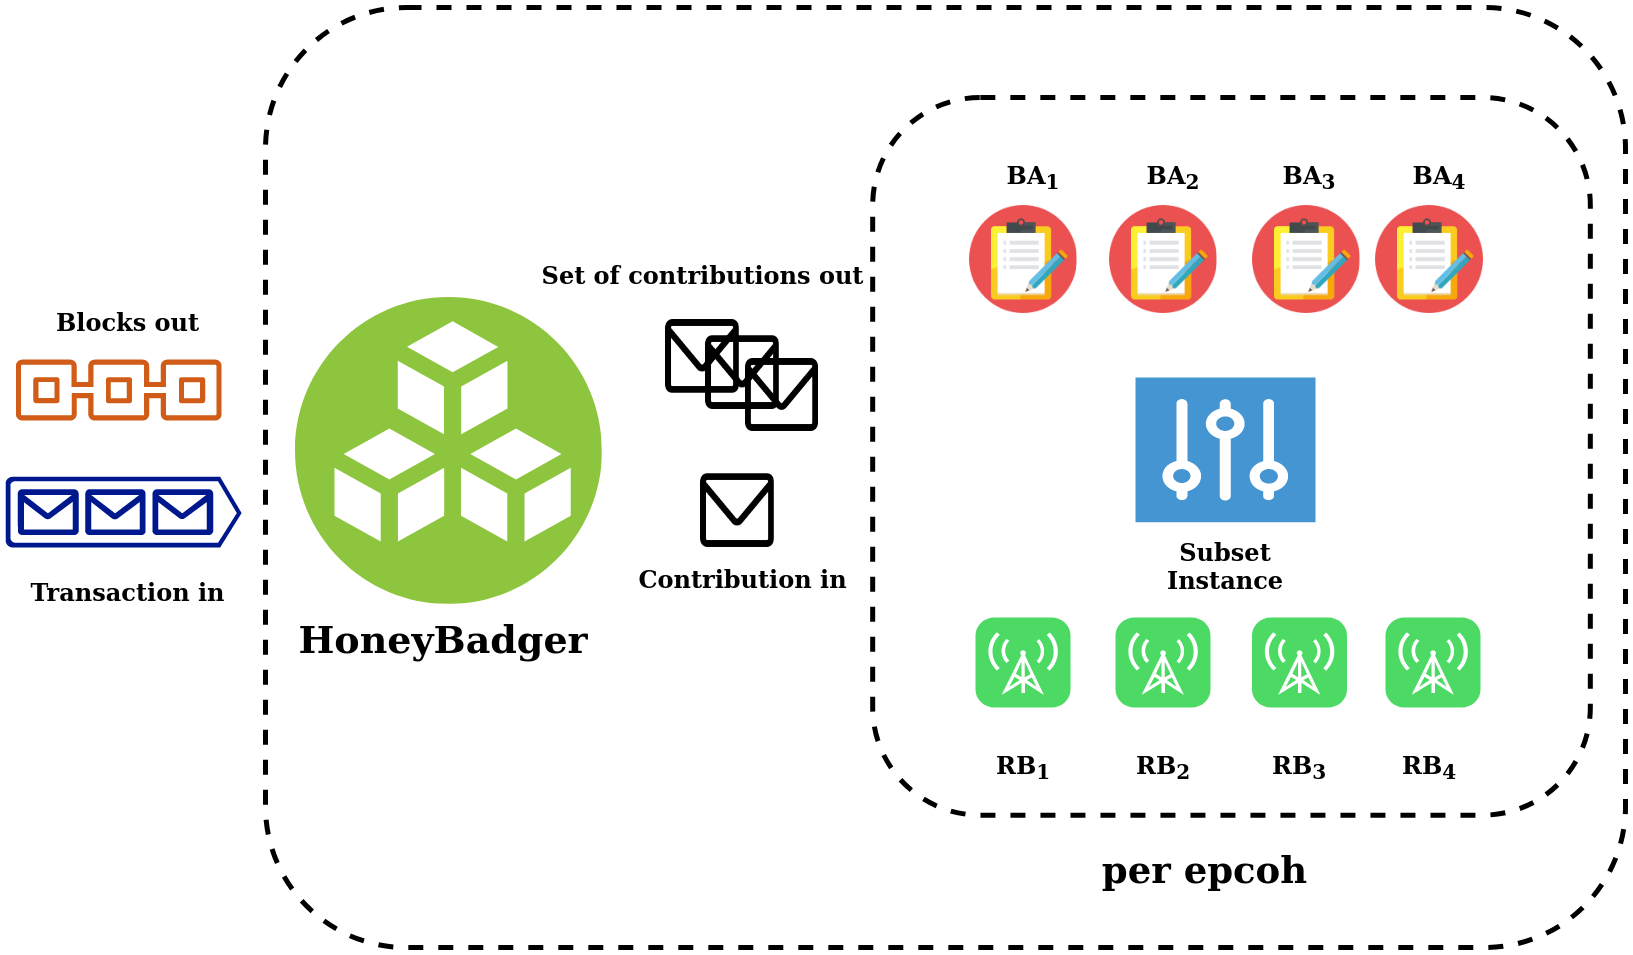
\includegraphics[width=1\textwidth]{images/hbbft_map.png}
    \caption{HoneyBadger component view for 4 nodes cluster}
    \label{fig:hbbft_map}
\end{figure}